\documentclass[conference]{IEEEtran}

\usepackage{amsmath,amssymb}
\usepackage{graphicx}
\usepackage{booktabs}
\usepackage{multirow}
\usepackage{cite}
\usepackage{url}
\usepackage{xcolor}
\usepackage{ctex}
\usepackage{array}
\usepackage{tabularx}
\usepackage{balance}

\begin{document}

\title{Prithvi-EO-2.0在海光K100 AI加速卡上的可审计混合精度部署：精度、内核路径与系统权衡}

\author{\IEEEauthorblockN{匿名作者}
\IEEEauthorblockA{匿名机构\\匿名地点\\anonymous@example.com}}

\maketitle

\begin{abstract}
地理空间基础模型的部署需要超越名义数据类型和文件压缩率的证据。本文给出一个面向特定硬件与运行时的可审计案例：将由Prithvi-EO-2.0-300M与UPerNet组成的约3.19亿参数洪水水体分割模型部署到海光K100 AI加速卡。验证链覆盖固定90幅影像上的任务效用、ONNX Runtime执行提供者放置、实际GEMM内核路径、同拓扑与same-CLI性能，以及不可变部署包的运行行为。实验建立25段FP32分母，并评估6个固定的诊断知情FP16/INT8配置M0--M5。M4取得混合精度中的最高实测mIoU（0.86037）；M5取得0.86027 mIoU和22.080 ms端到端logits中位时延，相比25段FP32的22.209 ms低约0.58\%，本文将其表述为时延持平，而非正式INT8加速。profile中MIGraphX事件为正且CPU提供者事件为0，trace进一步识别出INT8 block中的I8II GEMM和FP16 block中的HBH GEMM。然而，在生产式same-CLI比较中，M5比单体Full FP16慢73.642\%，尽管完整部署载荷减少23.463\%。两个部署包均通过5次冷启动、3次主动终止恢复、双节点冒烟测试和60分钟稳定性测试，未出现推理错误、非有限输出或预测漂移。对于本文评估的checkpoint与K100软件栈，Full FP16是速度优先的主部署方案，M5是存储优先的可部署备选。
\end{abstract}

\begin{IEEEkeywords}
地理空间基础模型，混合精度，部署验证，MIGraphX，海光K100
\end{IEEEkeywords}

\section{引言}
\label{sec:introduction}

地理空间基础模型（GeoFM）通过大规模预训练迁移到土地覆盖制图、变化检测和灾害响应等下游对地观测任务。Prithvi-EO-2.0在全球Harmonized Landsat与Sentinel-2时序数据上引入多时相和位置感知预训练~\cite{prithvi2024}；相关掩码自编码工作也证明了卫星影像光谱结构与时间结构的价值~\cite{satmae2022}。但是，这类模型通常具有数亿参数，实际部署图还包含Transformer编码器、归一化、多尺度特征重建和密集预测任务头。

低精度推理可以降低artifact容量，并可能暴露低精度内核，但任务保持、加速卡放置、实际算术路径和应用时延是不同主张。针对视觉Transformer的后训练量化研究处理激活分布、LayerNorm通道差异与尺度重参数化~\cite{ptq4vit2022,fqvit2022,repqvit2023}；硬件感知混合精度研究则强调转换开销和运行时约束~\cite{hawqv3}。因此，编译器融合、图划分、Q/DQ边界、布局转换和会话调度都可能抵消名义算术收益。

本文研究Prithvi-EO-2.0-300M与UPerNet~\cite{upernet2018}在海光K100 AI加速卡上的部署。\textit{本文不提出新的量化算法，也不提出可跨平台迁移的通用混合精度策略。}本文是一项面向特定硬件与运行时的部署案例研究。历史上失败的CPU/MIGraphX严格logits诊断被永久保留，同时另设应用级轨道评估不可变artifact在目标软件栈上的可用性。证据被组织为任务效用、提供者放置、实际内核、系统性能和运行可靠性五层。

本文的主要贡献如下：
\begin{enumerate}
    \item 提出一套五层可审计证据框架，将任务效用、提供者放置、实际内核、性能和运行可靠性分开，避免把名义INT8或压缩率直接当作部署成功。
    \item 建立设备驻留OrtValue传递的同拓扑25段FP32分母，使FP32与M0--M5的分段系统时延比较具有一致拓扑。
    \item 将不可变ONNX配置、提供者profile与逐block I8II/HBH trace关联起来：33个去重artifact trace支撑144个“候选--block”映射，profile中未观察到CPU提供者事件。
    \item 将M5和Full FP16封装为不可变部署包，并验证冷启动、主动恢复、跨节点执行、60分钟运行和生产式same-CLI比较。
\end{enumerate}

本文不声称混合图中的所有算子均为原生INT8，不声称CPU与MIGraphX logits严格等价，也不把INT8算术路径直接表述为整模型加速。

\section{相关工作}
\label{sec:related_work}

\subsection{地理空间基础模型与下游适配}

视觉Transformer（ViT）将图像切分为patch序列并使用自注意力进行表征学习~\cite{vit2021}。遥感掩码预训练随后引入多时相、多光谱、显式空间尺度及对齐的雷达--光学数据，SatMAE、Scale-MAE和CROMA是其中的代表~\cite{satmae2022,scalemae2023,croma2023}。RingMo与持续地理空间预训练扩展了跨传感器和下游任务的表征~\cite{ringmo2023,gfm2023}；SkySense与DOFA则研究多模态或传感器灵活的对地观测编码器~\cite{skysense2024,dofa2024}。Prithvi-EO-2.0进一步采用多时相与位置感知预训练并支持下游适配~\cite{prithvi2024}。本文不提出新骨干，而是研究一个已微调300M模型在目标加速卡上的精度变换与部署行为。

\subsection{Transformer的后训练量化与混合精度}

当量化语义与硬件内核匹配时，整数推理能够缩小模型并执行整数算术~\cite{jacob2018}。视觉Transformer PTQ研究排序保持校准、非高斯激活、LayerNorm通道差异和尺度重参数化~\cite{vitptq2021,ptq4vit2022,fqvit2022,repqvit2023}；硬件感知和敏感性知情的混合精度工作则依据设备反馈或层级信号分配位宽~\cite{haq2019,hawqv3,mixqvit2026}。本文既不提出PTQ方法，也不估计任务损失敏感性，而是依据同一冻结artifact在两个后端上的差异构建固定精度配置。

\subsection{硬件感知部署与运行时编译}

ONNX Runtime通过执行提供者抽象支持跨平台部署~\cite{onnxruntime}。MIGraphX对计算图进行编译和算子下沉，并通过融合等变换影响实际执行~\cite{migraphx}。可复现推理基准还需要明确场景、精度约束和计时定义，而不能依赖单个无上下文的时延值~\cite{mlperf2020}。但是，提供者被注册或排在首位，不等于算子确实落卡；算子落卡也不等于实际采用了整数内核。本文因此联合使用提供者profile、kernel trace和端到端测量，而不是用图中数据类型或文件大小代替加速证据。

\subsection{遥感模型的部署验证}

遥感压缩研究开始联合考虑模型大小、分辨率与任务精度~\cite{shinde2025}。面向真实系统的GeoFM工作进一步强调应用需求、领域适配和基准之外的经验验证~\cite{worldcereal2025}；PhiSat-1展示了受限对地观测场景中的星上深度学习验证~\cite{phisat2022}，近期综述则从模型优化、软件工具链和受限硬件三个方面组织星载遥感基础模型部署~\cite{sang2026}。这些工作共同说明，部署artifact必须可执行、可测量并可恢复，而不能只在离线框架中保持精度。

在本文审阅的研究范围内，尚未识别出一条同时报告任务效用、提供者放置、实际内核、同拓扑性能和目标GeoFM软件栈运行行为的完整评估链。本文联合报告这些证据层，同时把结论限制在所评估的checkpoint与K100软件栈。

\section{模型与部署方法}
\label{sec:method}

部署过程从冻结FP32参考模型出发，经后端差异诊断和固定精度配置后进入K100执行。证据链将任务效用、提供者放置、实际内核、系统性能和运行验收明确分开。

图~\ref{fig:framework_cn}概括不可变artifact流水线和用于形成部署决策的五层证据。该图描述的是审计结构而非新的量化算法：文件精度、提供者放置、实际内核精度、系统性能和运行可靠性仍是相互独立的主张。

\begin{figure*}[t]
\centering
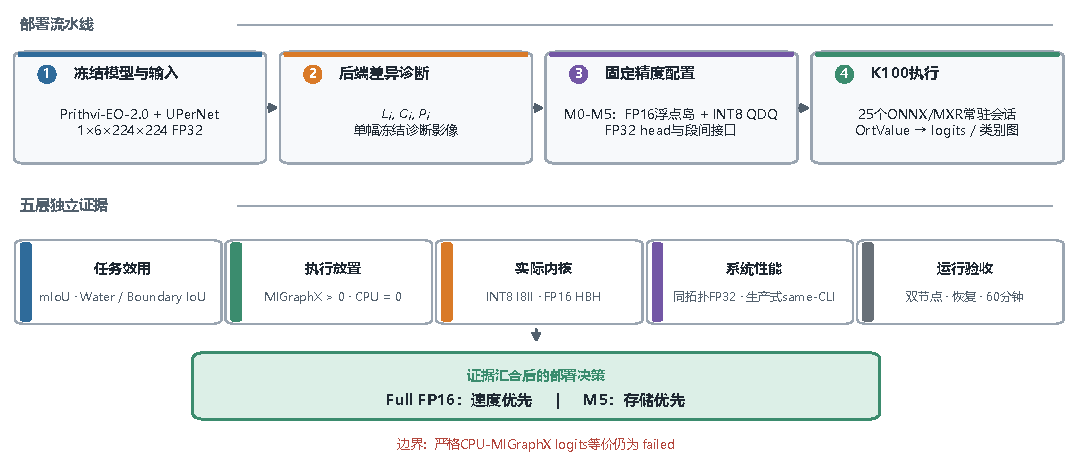
\includegraphics[width=0.98\textwidth]{figures/fig1_k100_framework_cn.pdf}
\caption{K100可审计部署总览。冻结模型与输入身份依次进入后端诊断、固定M0--M5精度映射和25个常驻ONNX/MXR会话；不可变artifact与五类证据保持分离，最终工程决策不能由名义数据类型直接推出。}
\label{fig:framework_cn}
\end{figure*}

\subsection{任务与冻结输入契约}

实验任务为Sen1Floods11~\cite{sen1floods11}二分类洪水水体分割。模型由Prithvi-EO-2.0-300M编码器和UPerNet解码器组成，总参数约3.19亿。评估固定使用公开测试集的90幅影像和3,927,398个有效像素。输入形状为$1\times6\times224\times224$，六个波段依次为BLUE、GREEN、RED、NIR\_NARROW、SWIR\_1和SWIR\_2。输入为经过数据集$10^{-4}$比例缩放后的有限FP32反射率张量；归一化已嵌入导出模型，部署客户端不得重复执行。

任务指标由全局混淆矩阵计算，包括mIoU、Water IoU、pixel accuracy和Boundary Water IoU。对于二值水体掩膜$m$，实现采用半径为2像素的形态学梯度：
\begin{equation}
\begin{aligned}
B(m)&=\delta_{2}(m)-\left[1-\delta_{2}(1-m)\right],\\
\operatorname{BIoU}&=\frac{|B(\hat m)\cap B(m)\cap V|}{|(B(\hat m)\cup B(m))\cap V|},
\end{aligned}
\label{eq:boundary-iou_cn}
\end{equation}
其中，$\delta_2$是步长为1、核为$5\times5$方形的max pooling，水体编码为类别1，$V$为target不等于ignore值的有效像素掩膜。交集与并集在90幅影像上全局累计；若全局并集为空，则报告未定义而不是人为赋值。早期artifact中的“corrected”表示修复了ignore mask广播：掩膜在应用前显式加入单例通道维，避免从$N\times H\times W$错误广播为$N\times N\times H\times W$。因此正文和表格统一称为Boundary Water IoU。相对冻结FP32的应用级准入标准为：mIoU下降不超过0.5个百分点（pp），Water IoU和Boundary Water IoU下降均不超过1.0 pp，有效像素预测一致率不低于99.5\%，且非有限输出为0。

\subsection{25段执行拓扑}

部署骨干由24个Transformer block段和1个UPerNet head段组成。所有段间接口统一为FP32，并通过设备驻留的ONNX Runtime OrtValue传递，避免相邻段之间回到主机内存。为适配目标编译器，必要的LayerNorm被展开，解码器ConvTranspose被重写，并在head中加入fpn4 MaxPool barrier以获得稳定的加速卡放置。每个ONNX段及其MXR编译缓存均具有冻结的独立身份。

FP32和混合精度候选采用相同的25段拓扑。单体FP32会话与25会话混合流水线具有不同的调度、缓存和段边界成本，因此本文只使用25段FP32作为同协议性能分母。

\subsection{后端差异定位}

配置序列并非只依据最终logits，而是通过显式逐段后端诊断获得。对于第$i$段，令$x_i^{C}$表示CPU参考链生成的输入，$x_i^{M}$表示MIGraphX累计链生成的输入，$f_i^{C}$与$f_i^{M}$分别表示同一冻结段artifact在CPU和MIGraphX上的执行。定义三个互补差异：
\begin{equation}
\begin{aligned}
L_i &= \operatorname{MAE}\!\left(f_i^{C}(x_i^{C}),f_i^{M}(x_i^{C})\right),\\
C_i &= \operatorname{MAE}\!\left(f_i^{C}(x_i^{C}),f_i^{M}(x_i^{M})\right),\\
P_i &= \operatorname{MAE}\!\left(f_i^{M}(x_i^{C}),f_i^{M}(x_i^{M})\right).
\end{aligned}
\label{eq:localization_cn}
\end{equation}
其中，$L_i$为相同输入条件下的局部CPU--MIGraphX差异，$C_i$为经过第$i$段后的整链累计差异，$P_i$表示上游漂移对同一个MIGraphX段输出的影响。除MAE外，还记录最大绝对差异和相对$\ell_2$差异。$L_i$、$C_i$和$P_i$均为后端差异诊断量：它们既不是纯FP32到INT8量化误差，也不是任务损失敏感性。

诊断使用公开测试集中的一幅冻结真实影像，并只为暴露段边界而在主机侧暂存中间张量。它不是性能实验，也没有改变正式部署的设备驻留协议。25个段仍全部要求MIGraphX事件大于0、CPU提供者事件为0。由于一幅公开测试影像参与了后端差异诊断和后续配置序列构建，90幅影像结果应被理解为固定部署验证案例，而不是对配置泛化能力的无偏留出估计。本文不声称所观察的block模式能够跨影像、checkpoint、任务或加速卡软件栈泛化。

segment 0需要单独解释。它直接接收六波段图像，在第一个Transformer block之前还包含从图像到token的前端，包括归一化和patch embedding。内部checkpoint将第一次明显分歧定位在patch-embedding卷积的反量化输出，MAE为0.1316；attention-score处MAE达到0.3404；第二个MLP投影处达到0.3792；最终segment输出为0.4239。只将patch embedding恢复为FP32虽然能降低误差，却不能消除差异，因此block 0的大误差不是由某一个卷积单独造成的。基于这一证据，候选设计保护整个第一段，而不是只保护单个算子。

\subsection{诊断知情的精度配置}

表~\ref{tab:candidates_cn}给出固定且可审计的配置序列，而不是自动搜索算法。M0将24个骨干block全部设为INT8，head保持FP32。M1将诊断影像中高差异的block 0保护为FP16；M2--M4依次加入block 14、17和18；M5将block 14--21整体设为FP16。FP16段使用FP16权重和激活，但保留FP32 LayerNorm统计岛，且所有Cast均封装在段内；INT8段保持冻结QDQ语义；head始终为FP32。

\begin{table}[t]
\caption{混合精度候选定义}
\label{tab:candidates_cn}
\centering
\footnotesize
\begin{tabular}{clcl}
\toprule
候选 & FP16骨干block & INT8 block & Head \\
\midrule
M0 & 无 & 0--23 & FP32 \\
M1 & 0 & 其余23层 & FP32 \\
M2 & 0、14 & 其余22层 & FP32 \\
M3 & 0、14、17 & 其余21层 & FP32 \\
M4 & 0、14、17、18 & 其余20层 & FP32 \\
M5 & 0、14--21 & 其余15层 & FP32 \\
\bottomrule
\end{tabular}
\end{table}

图~\ref{fig:sensitivity-map_cn}把实测后端差异分布与固定配置对应起来。M1--M4依次保护诊断影像中的离散峰值，而M5保护连续的后期高差异区域；FP32 head始终固定，以隔离骨干精度映射的影响。

\begin{figure*}[t]
\centering
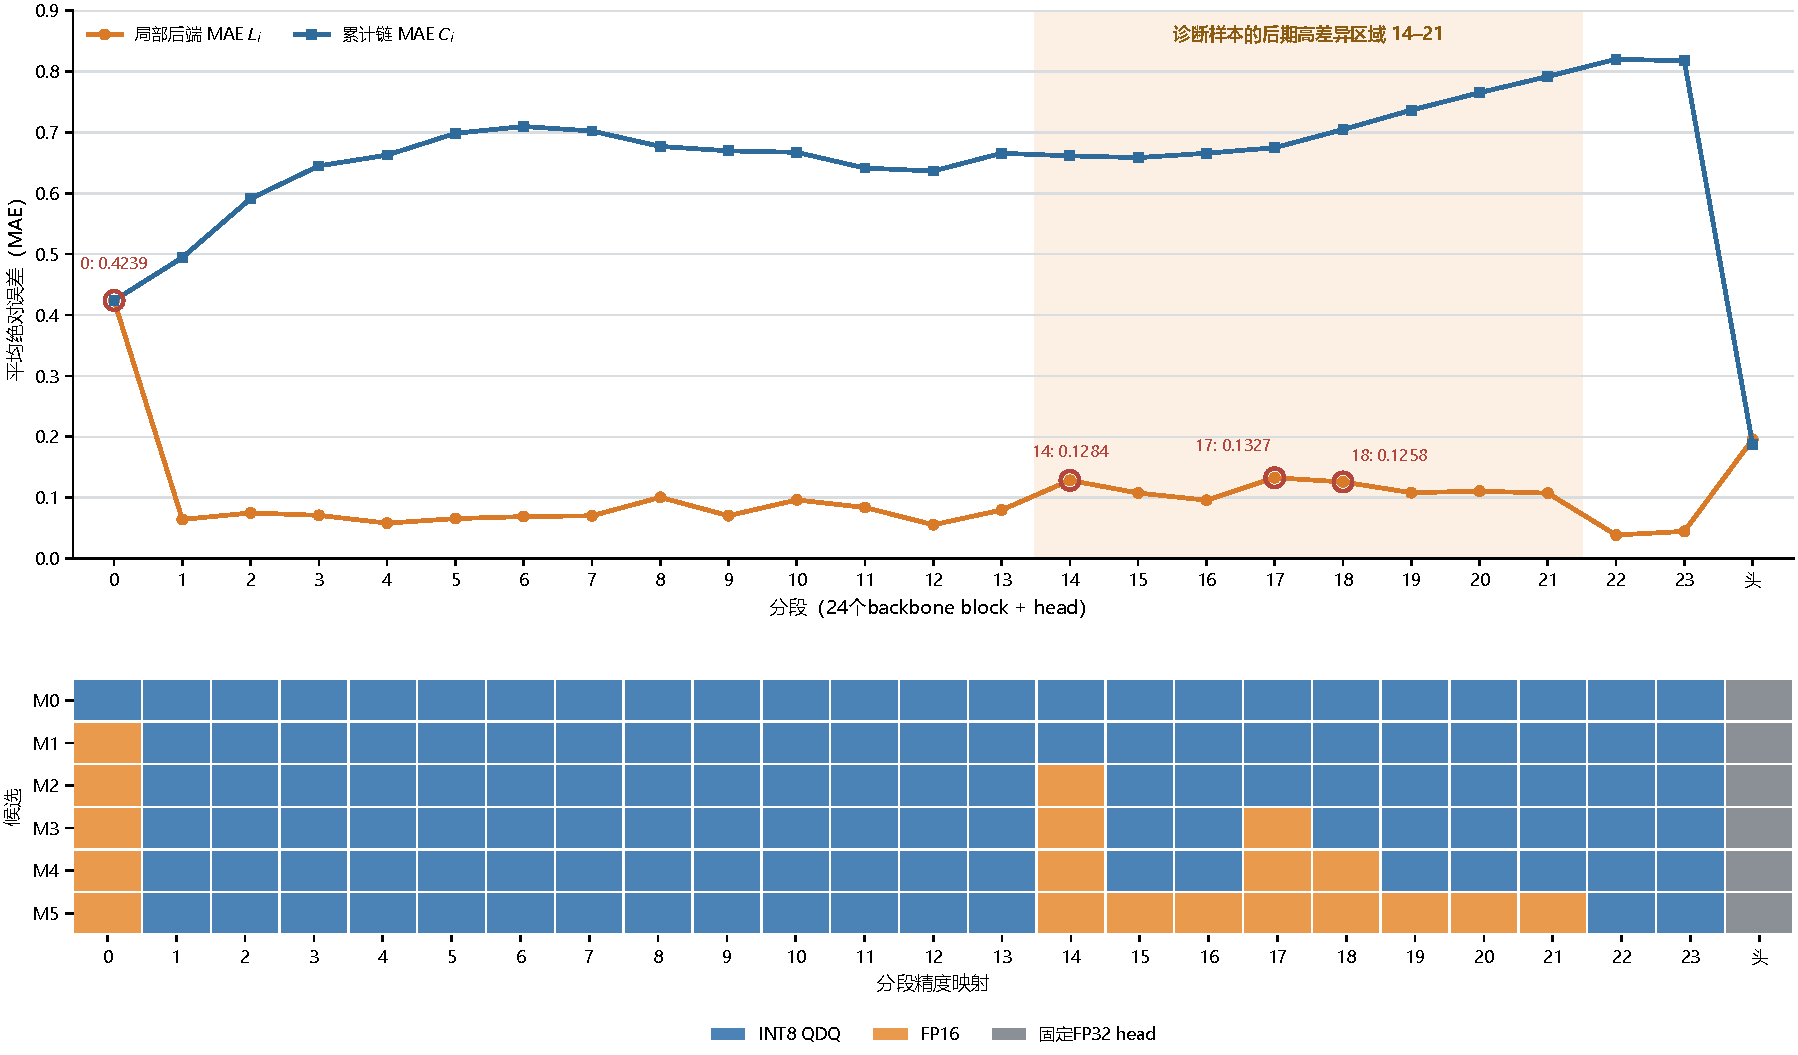
\includegraphics[width=0.98\textwidth]{figures/fig2_sensitivity_mapping_cn.pdf}
\caption{单幅诊断影像的CPU--MIGraphX后端差异profile及固定M0--M5精度映射。圆圈标记M1--M4使用的选定峰值，M5保护block 14--21；该profile具有案例特异性，不估计任务损失效应。}
\label{fig:sensitivity-map_cn}
\end{figure*}

\subsection{量化与模型转换细节}

源模型为使用TerraTorch 1.2.8训练的冻结Prithvi-EO-2.0-300M--UPerNet checkpoint（SHA-256前缀为\texttt{59f031}）。其FP32 ONNX以opset 17导出，输入\texttt{image}和输出\texttt{logits}分别为FP32 $[1,6,224,224]$与$[1,2,224,224]$，输入归一化已嵌入图中；导出一致性检查的最大绝对差异为$4.768\times10^{-6}$。冻结sidecar未保留精确PyTorch exporter版本，本文不作推断。

INT8段复用由ONNX Runtime quantization 1.26.0生成的不可变static-PTQ QDQ artifact；K100实验没有重新估计scale或zero point。激活和权重均使用signed INT8 Q/DQ张量（S8S8）；激活非对称、权重对称，权重采用per-channel、激活采用per-tensor。量化器实际选择的通道axis及解析后的scale/zero-point张量dtype没有在sidecar中单独保留，因此本文不重构这些字段。MinMax校准按数据集顺序使用官方训练集前64幅影像，执行确定性resize和$10^{-4}$输入缩放，不使用随机增强和标签。白名单为Conv、MatMul和Gemm；骨干artifact实际选中1个Conv与144个MatMul。LayerNorm、Softmax、残差Add、Resize及其他未选中算子保持浮点路径。Q/DQ对置于每段内部已选算子边界，UPerNet head和所有段外部接口均保持FP32。

冻结的Full FP16源artifact由\texttt{onnxconverter-common} 1.16.0转换，保留FP32外部I/O，包含332个FLOAT16 initializer，并在转换记录中修补48个attention Cast。抽取后的FP16段使用FP16权重与激活，但通过显式FP32岛计算LayerNorm统计量，Cast全部封装在段内。ONNX Runtime 1.19.2通过MIGraphX 5.1.0 Execution Provider将每个不可变ONNX段编译或加载为MXR缓存；下文以模型和缓存的size/SHA身份界定实际编译产物，而不猜测未记录的命令行。

\subsection{分层证据协议}

实验区分五条证据轨道。

\textit{任务轨道：}每个候选均在90个固定样本上使用3个新进程独立评估，由上述任务指标决定应用准入。

\textit{性能轨道：}只有任务准入通过后，才使用batch 1、30次预热、3个新进程、每进程100次正式测量。报告median、P95、P99、吞吐量和轮间median CV；CV超过5\%时禁止正式速度表述。

\textit{放置轨道：}每个段的profile必须满足MIGraphX事件大于0、CPU提供者事件等于0，且段间值保持在设备OrtValue中。

\textit{内核轨道：}利用hipprof识别每个去重block artifact的GEMM路径。INT8 block目标路径为I8II，FP16 block目标路径为HBH；Q/DQ、Cast、布局转换和Memcpy分别统计。

\textit{运行轨道：}部署包通过manifest SHA-256锁定，并执行冷启动、主动恢复、跨节点和60分钟连续运行测试。

此外，CPU与MIGraphX之间更严格的logits比较永久保留为非阻塞诊断。它不能覆盖任务证据，其失败结果将在第~\ref{sec:discussion_cn}节明确披露。

\section{实验设置}
\label{sec:setup_cn}

实验使用两台K100节点，核验环境见表~\ref{tab:environment_cn}。正式实验冻结容器镜像、运行时指纹、模型和缓存SHA、输入SHA、提供者profile以及原始时延数组。放置测试禁用隐式CPU fallback，并独立解析profile证据。

\begin{table*}[t]
\caption{硬件、软件与测量环境}
\label{tab:environment_cn}
\centering
\footnotesize
\begin{tabularx}{\textwidth}{>{\raggedright\arraybackslash}p{0.20\textwidth} X}
\toprule
类别 & 已核验配置 \\
\midrule
加速卡 & K100 AI加速卡；2个节点；\texttt{hy-smi}观测设备显存65,520 MiB。 \\
主机操作系统 & Ubuntu 20.04 LTS；Linux 5.4.0-216-generic。 \\
主机内存 & 可见内存62 GiB。 \\
容器镜像 & Ubuntu 22.04.5；镜像\texttt{sha256:bdc7e817...17b01}。 \\
语言/框架 & Python 3.10.12；PyTorch 2.5.1；HIP 6.3.25405。 \\
编译器/运行时 & DTK 25.04.2；MIGraphX 5.1.0+\texttt{das.opt1.dtk25042}；ONNX Runtime 1.19.2+\texttt{das.opt1.dtk25042}。 \\
运行策略 & Batch 1；观测为动态/auto性能模式；预检时无其他K100任务。 \\
计时方法 & 主机\texttt{perf\_counter\_ns}；I/O binding显式同步输入，并在结束时同步最终输出。 \\
重复协议 & 30次预热；3个新进程$\times$100次正式测量。 \\
Model-only范围 & 设备驻留输入OrtValue到设备驻留logits。 \\
端到端logits范围 & 外部FP32输入传输、推理到最终logits回传主机。 \\
吞吐量定义 & Batch 1下为$N\times1000/\sum_j t_j$ sample/s，其中$t_j$的单位为ms。 \\
增量显存定义 & 独立新进程；\texttt{mem\_info\_vram\_used}峰值减去20个空闲基线样本的中位数；目标轮询间隔10 ms。 \\
运行遥测 & 稳定性测试每5 s采样温度、功耗与显存。 \\
输入契约 & FP32 $1\times6\times224\times224$；有限值；固定六波段顺序。 \\
\bottomrule
\end{tabularx}
\end{table*}

系统性能区分两个口径。\textit{Model-only}以已经驻留设备的输入OrtValue为起点，并将logits留在设备；\textit{端到端logits}使用公共推理harness完成外部输入到logits的路径。最后的配对比较让M5和Full FP16通过同一个公共CLI和同一个\texttt{K100BundleRunner.run}代码路径执行。

完整部署包接受形状为$1\times6\times224\times224$的有限FP32张量，输出形状为$1\times2\times224\times224$的FP32 logits和uint8类别图。非法shape、dtype或NaN/Inf直接失败，不进行静默转换。

\subsection{比较范围}

表~\ref{tab:scope_cn}明确区分全文使用的三种比较范围。所有结论仅在对应范围内解释，不能跨不同图拓扑或CLI路径推导“纯精度加速”。

\begin{table*}[t]
\caption{比较范围与允许解释}
\label{tab:scope_cn}
\centering
\small
\begin{tabular}{p{0.16\textwidth}p{0.24\textwidth}p{0.24\textwidth}p{0.22\textwidth}}
\toprule
范围 & 比较artifact & 受控接口 & 允许解释 \\
\midrule
同拓扑 & 25段FP32与M0--M5 & 相同25会话、设备驻留OrtValue拓扑 & 分段系统时延与运行重复性 \\
Same-CLI & 最终M5部署包与单体Full FP16 & 相同固定输入与\texttt{K100BundleRunner.run}路径 & 生产式部署决策，不能隔离算术精度影响 \\
存储 & ONNX+MXR逻辑容量与完整部署包载荷 & 分别定义并按字节统计 & 仅用于容量比较，不推导时延 \\
\bottomrule
\end{tabular}
\end{table*}

\subsection{可复现性与Artifact追溯}

每项正式结果均关联不可变ONNX与MXR SHA-256、固定输入hash、容器digest、运行时指纹和配置manifest。项目证据包还保留原始时延数组、提供者profile、kernel trace、完整bundle manifest、静态校验receipt和排除账本；失败启动被单独保存，不会被静默改写为通过。上述材料随项目证据包保留，本文不声称artifact已经公开发布。

\section{实验结果}
\label{sec:results_cn}

\subsection{逐层后端差异分布}

表~\ref{tab:localization_cn}给出完整逐段定位结果，并显示三种关键模式。第一，segment 0是最早且最大的局部CPU--MIGraphX分歧：$L_0=0.4239$，相对$\ell_2=0.2978$；由于两条链从完全相同的图像开始，$P_0=0$。因此，该段产生的后端差异可能进入后续残差流。第二，block 14--21形成后期高差异区域，其中14、17、18是最明显的局部峰值，而15、16、19--21仍处于中等偏高水平。M2--M4依次加入三个峰值；M5则保护完整的14--21连续区域，用于比较连续区域保护与孤立峰值保护的部署结果。

\begin{table*}[t]
\caption{冻结真实样本上的逐段CPU--MIGraphX后端差异定位}
\label{tab:localization_cn}
\centering
\scriptsize
\begin{tabular}{crrrrl@{\qquad}crrrrl}
\toprule
段 & $L_i$ MAE & 局部max & 相对$\ell_2$ & $C_i$ MAE & 精度作用 & 段 & $L_i$ MAE & 局部max & 相对$\ell_2$ & $C_i$ MAE & 精度作用 \\
\midrule
\textbf{0} & \textbf{0.4239} & \textbf{3.5917} & \textbf{0.2978} & 0.4239 & M1--M5 FP16 & 13 & 0.0797 & 0.4972 & 0.0507 & 0.6658 & INT8 \\
1 & 0.0642 & 1.4324 & 0.0459 & 0.4944 & INT8 & \textbf{14} & \textbf{0.1284} & 0.7954 & \textbf{0.0815} & 0.6615 & M2--M5 FP16 \\
2 & 0.0749 & 0.9584 & 0.0478 & 0.5913 & INT8 & 15 & 0.1076 & 0.5345 & 0.0663 & 0.6586 & M5 FP16 \\
3 & 0.0709 & 1.1014 & 0.0440 & 0.6450 & INT8 & 16 & 0.0958 & 0.9325 & 0.0587 & 0.6658 & M5 FP16 \\
4 & 0.0581 & 2.6298 & 0.0396 & 0.6628 & INT8 & \textbf{17} & \textbf{0.1327} & 1.2882 & \textbf{0.0807} & 0.6749 & M3--M5 FP16 \\
5 & 0.0656 & 0.7842 & 0.0409 & 0.6985 & INT8 & \textbf{18} & \textbf{0.1258} & 0.8274 & \textbf{0.0731} & 0.7048 & M4--M5 FP16 \\
6 & 0.0689 & 0.6987 & 0.0421 & 0.7098 & INT8 & 19 & 0.1081 & 0.8140 & 0.0616 & 0.7366 & M5 FP16 \\
7 & 0.0702 & 0.7861 & 0.0418 & 0.7023 & INT8 & 20 & 0.1107 & 0.6298 & 0.0622 & 0.7653 & M5 FP16 \\
8 & 0.1005 & 0.6774 & 0.0621 & 0.6770 & INT8 & 21 & 0.1074 & 0.6207 & 0.0582 & 0.7919 & M5 FP16 \\
9 & 0.0703 & 0.7109 & 0.0440 & 0.6697 & INT8 & 22 & 0.0386 & 0.2541 & 0.0199 & 0.8203 & INT8 \\
10 & 0.0963 & 1.7752 & 0.0609 & 0.6673 & INT8 & 23 & 0.0446 & 0.4270 & 0.0190 & 0.8176 & INT8 \\
11 & 0.0838 & 0.7812 & 0.0542 & 0.6414 & INT8 & Head & 0.1957 & 0.7799 & 0.1174 & 0.1871 & 固定FP32 \\
12 & 0.0554 & 1.0831 & 0.0401 & 0.6366 & INT8 & & & & & & \\
\bottomrule
\end{tabular}
\vspace{2pt}
\parbox{0.96\textwidth}{\scriptsize $L_i$表示同输入局部CPU--MIGraphX MAE，$C_i$表示累计链MAE。它们不是纯量化误差或任务损失敏感性。粗体为M1--M4依次使用的峰值block；M5进一步保护连续区域中的15、16和19--21。主机暂存诊断中的计时不属于性能证据。}
\end{table*}

第三，局部误差和累计误差均不随深度单调变化。block 22和23具有最小的两个局部相对$\ell_2$误差（0.0199和0.0190），但累计MAE仍超过0.81，因为它们继承了前面已经形成的漂移。相反，block 7--13即使引入非零局部误差，累计误差也会阶段性下降。原因在于误差是带方向的向量而不是只能逐层相加的非负标量；残差相加、归一化、注意力混合和MLP投影都可能旋转、衰减或放大已有扰动。

局部最大值也必须与MAE和相对$\ell_2$联合解释。block 4的最大差异达到2.6298，但MAE只有0.0581，说明主要是稀疏离群值，而不是广泛失真。block 14的最大值较小，但MAE和相对$\ell_2$明显更高，因此被纳入FP16保护配置。FP32 head的局部提供者差异也较高，但多尺度特征映射为两个logits后，累计输出MAE降至0.1871。Head通过独立的fpn4-barrier兼容性修复处理，不被计作INT8骨干block。

\subsection{严格跨提供者Logit诊断}

表~\ref{tab:strict-logits_cn}永久保留同一冻结artifact在单幅真实输入上的CPU与MIGraphX FP32输出logits诊断。预定义严格跨提供者诊断容差为MAE不超过$10^{-3}$、最大绝对误差不超过$5\times10^{-2}$、像素类别一致率不低于99.9\%。这些阈值用于诊断严格跨提供者可互换性，与90幅影像的应用级分割门槛相互独立。

\begin{table*}[t]
\caption{一幅冻结真实输入上的严格CPU--MIGraphX Logit诊断}
\label{tab:strict-logits_cn}
\centering
\small
\begin{tabular}{lrrrll}
\toprule
Artifact & MAE & 最大绝对误差 & 类别一致率 & 预定义容差 & 状态 \\
\midrule
Full FP16 & 0.003715 & 0.013458 & 100.0000\% & $10^{-3}/5\!\times\!10^{-2}/99.9\%$ & failed（MAE） \\
M0 & 0.110935 & 0.609328 & 99.9960\% & 同上 & failed \\
M1 & 0.126587 & 0.473313 & 100.0000\% & 同上 & failed \\
M2 & 0.094231 & 0.407406 & 100.0000\% & 同上 & failed \\
M3 & 0.104744 & 0.387089 & 100.0000\% & 同上 & failed \\
M4 & 0.108455 & 0.393831 & 100.0000\% & 同上 & failed \\
M5 & 0.092546 & 0.388980 & 100.0000\% & 同上 & failed \\
\bottomrule
\end{tabular}
\end{table*}

该诊断失败在证据记录中永久保留，它禁止严格logits等价或跨提供者校准可互换的claim。论文的应用部署准入则依据冻结90幅影像的分割指标与运行验收，因此该诊断不作为应用级阻塞项。

\subsection{任务效用}

表~\ref{tab:task_cn}给出冻结的90样本结果。同拓扑FP32完全复现参考任务指标；Full FP16的mIoU仅下降0.0131 pp。M0--M5全部在3个独立进程中通过预注册的应用级任务门槛，且三轮指标跨度均为0。该重复性只说明固定样本与冻结运行协议下的确定性，不能替代跨场景统计置信区间。M4具有最高的混合精度mIoU和Water IoU；M5精度略低于M4，但仍接近FP32，并在后续性能与部署分析中体现容量价值。

\begin{table*}[t]
\caption{固定90样本上的任务指标}
\label{tab:task_cn}
\centering
\small
\resizebox{\textwidth}{!}{%
\begin{tabular}{lccccccl}
\toprule
变体 & mIoU & Water IoU & Boundary Water IoU & Pixel Acc. & 一致率 & 骨干block（FP32/FP16/INT8） & 状态 \\
\midrule
FP32 & 0.860587 & 0.757838 & 0.362581 & 0.967110 & 100.0000\% & 24/0/0 & 参考 \\
Full FP16 & 0.860456 & 0.757588 & 0.361931 & 0.967094 & 99.9812\% & 0/24/0 & 通过 \\
M0 & 0.859288 & 0.755400 & 0.361058 & 0.966947 & 99.7071\% & 0/0/24 & 通过 \\
M1 & 0.860324 & 0.757386 & 0.362813 & 0.967077 & 99.8789\% & 0/1/23 & 通过 \\
M2 & 0.860044 & 0.756883 & 0.362193 & 0.967050 & 99.8731\% & 0/2/22 & 通过 \\
M3 & 0.860228 & 0.757201 & 0.362100 & 0.967065 & 99.8767\% & 0/3/21 & 通过 \\
M4 & 0.860371 & 0.757470 & 0.362530 & 0.967085 & 99.8753\% & 0/4/20 & 通过 \\
M5 & 0.860272 & 0.757295 & 0.362517 & 0.967029 & 99.8781\% & 0/9/15 & 通过 \\
\bottomrule
\end{tabular}
}
\parbox{0.98\textwidth}{\footnotesize FP32与M0--M5的UPerNet head保持FP32。Full FP16遵循正式部署的单体兼容图：内部FP16参数/激活、FP32岛和FP32外部I/O。所有行均聚合同一90幅影像与3,927,398个有效像素。}
\end{table*}

M0到M1的提升与block 0较大的后端差异一致：只保护这一段便恢复了大部分任务指标损失。后续FP16替换并没有形成单调的指标序列；残差路径会衰减或放大扰动，解码器又会读取多个深度的特征。因此，逐段后端差异只能用于构造待验证配置，不能被解释为单层任务因果效应，也不能据此机械排序。

图~\ref{fig:flood-qualitative_cn}为全局指标提供空间层面的补充。在稀疏水体场景中，三条执行路径都漏掉了大部分零散小水体；在中等和大范围水体场景中，误检与漏检主要集中于狭窄岸线和破碎边界，而Full FP16与M5对主体水体几何形状的保持接近同拓扑FP32。该图用于展示误差形态，不构成新的精度估计。

\subsection{逻辑容量与压缩效果}

表~\ref{tab:capacity_cn}比较可执行模型与编译缓存容量。分段FP32分母由25个ONNX文件和25个MXR缓存组成，合计2,691,090,617字节（2566.424 MiB）；M0--M5采用相同的25段统计方法。Full FP16则统计其正式部署使用的单体ONNX与一个配对MXR缓存。对于候选$i$，节省容量定义为$S_{\mathrm{FP32}}-S_i$，缩减比例为$(1-S_i/S_{\mathrm{FP32}})\times100\%$，压缩倍数为$S_{\mathrm{FP32}}/S_i$。Full FP16容量为1284.756 MiB，相对FP32缩减49.940\%，压缩倍数为1.998$\times$。M0最小，为763.951 MiB和3.359$\times$；M5因保留更多FP16高差异block，容量为981.759 MiB，压缩倍数为2.614$\times$。这说明浮点保护以一定容量为代价换取任务精度，但所有混合候选相对分段FP32仍至少缩减61\%以上。

\begin{table*}[t]
\caption{不同混合精度相对同拓扑FP32的ONNX+MXR逻辑容量与压缩效果}
\label{tab:capacity_cn}
\centering
\small
\resizebox{\textwidth}{!}{%
\begin{tabular}{llrrrrrr}
\toprule
方案 & Backbone精度映射 & ONNX (MiB) & MXR (MiB) & 合计 (MiB) & 相对FP32节省 (MiB) & 缩减比例 & 压缩倍数 \\
\midrule
FP32 & 24个FP32块 & 1218.134 & 1348.290 & 2566.424 & 0.000 & 0.000\% & 1.000$\times$ \\
Full FP16 & 单体FP16 & 609.370 & 675.386 & 1284.756 & 1281.668 & 49.940\% & 1.998$\times$ \\
M0 & 0个FP16 + 24个INT8块 & 350.990 & 412.960 & 763.951 & 1802.473 & 70.233\% & 3.359$\times$ \\
M1 & 1个FP16 + 23个INT8块 & 364.016 & 425.362 & 789.378 & 1777.046 & 69.242\% & 3.251$\times$ \\
M2 & 2个FP16 + 22个INT8块 & 375.936 & 437.417 & 813.353 & 1753.071 & 68.308\% & 3.155$\times$ \\
M3 & 3个FP16 + 21个INT8块 & 387.856 & 449.666 & 837.522 & 1728.903 & 67.366\% & 3.064$\times$ \\
M4 & 4个FP16 + 20个INT8块 & 399.776 & 461.913 & 861.689 & 1704.735 & 66.425\% & 2.978$\times$ \\
M5 & 9个FP16 + 15个INT8块 & 459.375 & 522.384 & 981.759 & 1584.665 & 61.746\% & 2.614$\times$ \\
\bottomrule
\end{tabular}
}
\end{table*}

上述数值描述一个可执行配置的ONNX+MXR逻辑载荷，不包含容器镜像、Python与运行时依赖、文件系统实际占用，也不计入不同候选之间的硬链接共享。Full FP16为单体拓扑，而FP32与M0--M5为分段拓扑，因此该行只用于存储容量比较，不用于同拓扑执行性能比较。这些数值也不能与后文的完整部署bundle容量直接混用。

\begin{figure}[!t]
\centering
\makebox[\columnwidth][c]{%
  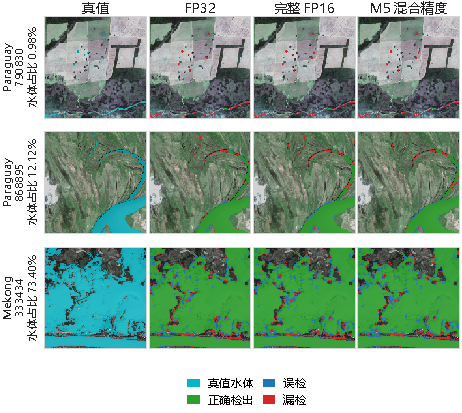
\includegraphics[width=0.96\columnwidth]{figures/fig_flood_qualitative_cn.pdf}%
}
\caption{三个固定测试场景上的洪水水体定性检测结果。样本在所有含有效水体像素的真值掩膜中，按有效像素水体占比的第25、第75和第95百分位独立确定，选择过程不使用模型精度。青色表示真值水体；预测行在RED--GREEN--BLUE合成影像上以绿色表示正确检出、蓝色表示误检、红色表示漏检。该图仅作定性展示，不能替代表~\ref{tab:task_cn}的90幅影像量化指标。}
\label{fig:flood-qualitative_cn}
\end{figure}

图~\ref{fig:tradeoff_cn}用两个面板区分不同范围的权衡。左侧仅比较同为25段拓扑的FP32与M0--M5；右侧单独给出最终部署包的same-CLI结果。这样既能展示INT8占比较高的候选更紧凑，也不会把单体Full FP16与25段配置混成精度专属的硬件加速比。

\begin{figure*}[t]
\centering
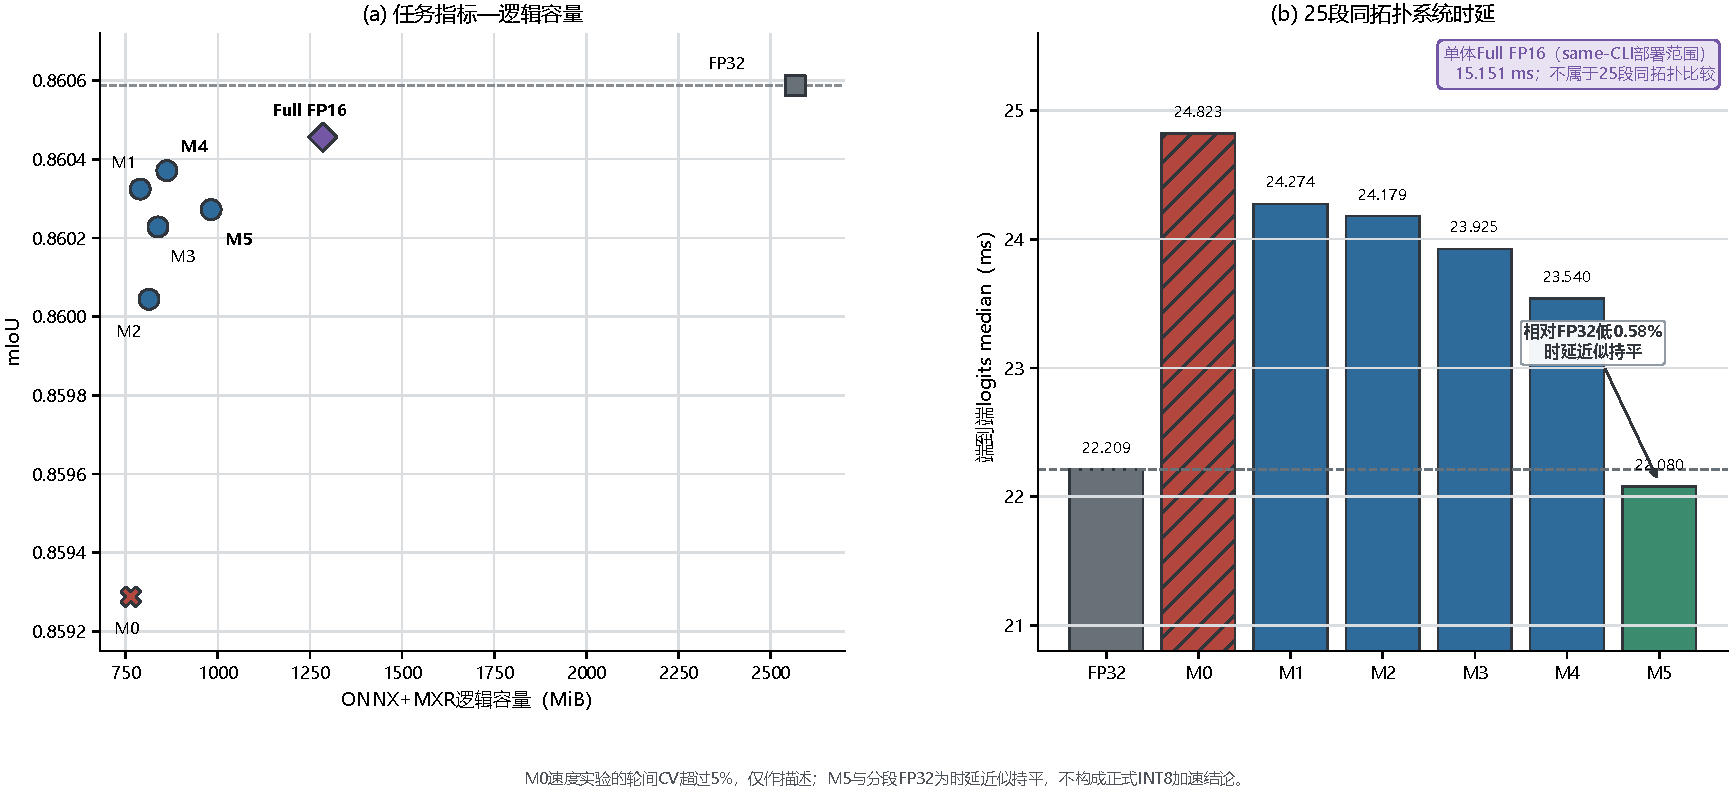
\includegraphics[width=0.82\textwidth]{figures/fig3_tradeoff_cn.pdf}
\caption{任务精度、逻辑容量与系统时延的分范围权衡。左：同拓扑25段FP32与M0--M5；右：最终M5与单体Full FP16部署包的same-CLI结果。两个面板采用不同执行范围，不能合并推导精度专属加速比。}
\label{fig:tradeoff_cn}
\end{figure*}

\subsection{同拓扑性能}

表~\ref{tab:performance_cn}只比较采用相同25段常驻会话拓扑的FP32与M0--M5。M1--M4尽管含有INT8 block，实际均慢于FP32。M5与FP32近似持平：端到端logits median分别为22.080 ms和22.209 ms，差约0.58\%。由于差值很小，且M5的尾延迟并未优于FP32，本文不将其表述为正式INT8加速。M0原始model-only轮间CV为6.47\%，因此保持unstable；后续确认实验只作为追加观测，不能覆盖这一冻结事实。

\begin{table*}[t]
\caption{25段配置的同拓扑性能（Batch 1，30次预热，$3\times100$次）}
\label{tab:performance_cn}
\centering
\small
\resizebox{\textwidth}{!}{%
\begin{tabular}{lcccccc}
\toprule
变体 & Model-only median & 端到端logits median & 速度因子 $T_{\mathrm{FP32}}/T_{\mathrm{variant}}$ & 增量显存 & CV状态 & 解释 \\
 & (ms) & (ms) &  & (GiB) & & \\
\midrule
FP32 & 21.349 & 22.209 & 1.000$\times$ & 19.230 & 通过 & 同协议分母 \\
M0 & 24.136 & 24.823 & 0.895$\times$ & 17.200--17.400 & 不稳定 & 最大压缩 \\
M1 & 23.550 & 24.274 & 0.915$\times$ & 17.200--17.400 & 通过 & 紧凑稳定 \\
M2 & 23.411 & 24.179 & 0.919$\times$ & 17.200--17.400 & 通过 & 慢于FP32 \\
M3 & 23.118 & 23.925 & 0.928$\times$ & 17.200--17.400 & 通过 & 慢于FP32 \\
M4 & 22.829 & 23.540 & 0.944$\times$ & 17.200--17.400 & 通过 & 精度优先 \\
M5 & 21.339 & 22.080 & 1.006$\times$ & 17.200--17.400 & 通过 & 时延持平；不作加速claim \\
\bottomrule
\end{tabular}
}
\parbox{\textwidth}{\footnotesize 注：速度因子大于1表示中位时延低于分段FP32，小于1表示更高；只在相同25段拓扑内计算。M5的1.006$\times$按时延持平处理，不构成正式加速claim。Full FP16的生产式same-CLI结果单独列于表~\ref{tab:cli_cn}。}
\end{table*}

因此，Pareto分析保留多个具有不同作用的候选，而不是强行选择一个“最佳INT8模型”：M0是最大压缩候选，但原始时序状态保持不稳定；M1是恢复M0大部分任务退化且满足时序稳定门槛的首个紧凑稳定配置；M4是精度取向混合点；M5是分段时延取向点和最终存储取向部署备选。Full FP16继续作为生产式部署速度参照，它与M5的正式配对结果单独列于表~\ref{tab:cli_cn}。

\subsection{内核与放置证据}

所有通过准入的候选均满足25个段MIGraphX事件大于0、CPU提供者事件为0。Kernel分析覆盖33个去重trace，其中包含24个INT8身份和9个FP16身份，并展开为144个“候选--block”映射。在本文冻结artifact与trace协议中，所有保留的INT8 block均观察到I8II GEMM路径，所有FP16 block均观察到HBH路径。

这比检查ONNX数据类型更接近实际硬件证据，但仍只是block级GEMM路径证据。FP32 head、LayerNorm浮点岛、Q/DQ、Cast、布局转换和数据复制仍属于完整流水线；trace还包含会话与MXR加载以及输入输出传输。因此，该结果不证明全图所有算子均为整数，也不能单独证明模型级加速。

\subsection{部署容量与same-CLI对比}

M5部署包包含74个payload文件，总计1,032,911,027字节；Full FP16包含19个payload文件，总计1,349,558,844字节。M5完整部署载荷减少316,647,817字节，即23.463\%。该完整bundle口径包含可执行产物、manifest、工具和固定验证数据，既不同于仅统计ONNX文件的压缩率，也不同于表~\ref{tab:capacity_cn}中的ONNX+MXR逻辑容量。

最终配对实验使用相同公共CLI、固定输入、runner实现和$3\times100$协议。表~\ref{tab:cli_cn}表明，尽管M5更小并含有已验证的INT8 GEMM，它仍显著慢于Full FP16。这是最终部署选择的决定性证据。

\begin{table}[t]
\caption{最终部署包的生产式same-CLI比较}
\label{tab:cli_cn}
\centering
\footnotesize
\begin{tabular}{lrrrr}
\toprule
部署包 & Median & P95 & P99 & 吞吐量 \\
 & (ms) & (ms) & (ms) & (sample/s) \\
\midrule
M5 & 26.309 & 28.518 & 30.744 & 37.641 \\
Full FP16 & 15.151 & 15.552 & 17.594 & 65.900 \\
\bottomrule
\end{tabular}
\vspace{2pt}
\parbox{0.96\columnwidth}{\footnotesize M5/FP16 median时延比为1.7364，M5慢73.642\%。M5和FP16的轮间median CV分别为0.413\%和0.086\%。该比较同时改变图拓扑与精度映射，只能用于最终部署决策，不能解释为纯INT8/FP16算术峰值排名。}
\end{table}

\subsection{运行验收}

两个不可变部署包均通过完整静态校验，包括manifest与payload哈希、运行时指纹、输入输出契约和固定向量预测。二者均通过5次冷启动和3次主动终止后重载。M5和FP16的session加载中位时间分别为8.883 s和10.086 s，runner初始化总时间分别为10.281 s和11.570 s；这些属于启动指标，不作为稳态吞吐证据。

两个部署包均在K100-2和K100-3通过带外层启动环境证明的正式冒烟测试。60分钟连续运行中，M5完成123,106次推理，FP16完成193,634次推理；每个测试均保存720条遥测，且崩溃、推理错误、非有限输出和固定样本预测漂移全部为0。M5温度范围为41--67$^{\circ}$C、功耗范围为108--217 W；FP16温度范围为43--59$^{\circ}$C、功耗范围为109--202 W。此前两次K100-3无效环境尝试和一次外层证明工具失败均通过排除账本保留，均不计入正式验收，且没有一次到达成功模型推理。

\section{讨论}
\label{sec:discussion_cn}

\subsection{后端差异诊断的解释}

逐段结果表明，CPU--MIGraphX差异并不随深度单调累积。segment 0同时包含输入前端与第一个Transformer block，较大的局部差异会进入后续残差流；block 14--21则形成第二个高差异区域。残差相加、归一化、注意力混合和MLP投影都可能改变扰动的方向与幅度，任务头还会消费多个深度的特征。因此，$L_i$或$C_i$不能直接等同于任务损失敏感性。M0、M1、M4和M5分别是固定的最大压缩、紧凑稳定、精度取向和分段时延取向消融点；最终判断仍来自完整90样本任务评估。

\subsection{为什么已验证的INT8内核不保证端到端加速}

M5已经满足逐block I8II证据，但在same-CLI下仍输给单会话Full FP16。该现象与多会话调度、段边界、Q/DQ、FP32段间接口、Cast、布局变换、FP32 head和剩余浮点算子的组合影响一致。当前实验没有单独计时这些部分，因此不把时延差距中的任何数值比例归因于某一来源。“存在INT8内核”与“应用系统变快”仍是两个必须分别取证的主张。

\subsection{部署含义}

所有部署候选均通过应用级分割门槛，并在三轮90样本评估中保持稳定。但是，历史CPU/MIGraphX严格logits诊断对INT8与混合精度artifact仍保持failed，本文不隐藏或改写该结果。因此，证据支持的是：在冻结数据与指标协议下，分割任务得到保持，artifact可在目标K100软件栈上可靠执行；证据不支持逐位等价或严格跨提供者logits复现。对于依赖概率校准、阈值敏感决策或跨后端精确复现的应用，仍需额外验证。

运行层面，M5与Full FP16均通过静态完整性、冷启动、恢复、双节点冒烟和60分钟稳定性验收，说明二者都具备操作性部署资格。容量与性能则给出不同取向：M5完整部署载荷少23.463\%，但same-CLI时延高73.642\%。因此，“能够部署”与“应当作为默认方案”必须分开表述。

\subsection{有效性威胁}

\textit{内部有效性：}校准使用官方训练集64幅影像，但没有为配置选择保留独立split。M0--M5的构造使用了一幅公开测试影像，随后又在包含该影像的固定90样本上评估，因此存在配置选择偏差；该实验是部署案例验证，而不是无偏的配置泛化估计。

\textit{构念有效性：}提供者事件为0只能说明profile中未观察到CPU执行；I8II/HBH只证明所跟踪GEMM路径，不代表整图所有算子均采用相应精度。ONNX+MXR逻辑容量与完整bundle载荷是不同构念，严格logits等价与任务指标保持也是不同目标。

\textit{外部有效性：}结论针对一个Prithvi-EO-2.0分割checkpoint、Sen1Floods11固定测试集、batch 1、两台K100节点以及当前DTK/MIGraphX/ONNX Runtime组合。25段图是兼容性策略，不代表其他模型、任务、batch、节点或软件版本的最优实现。

\textit{结论有效性：}三个新进程只刻画运行重复性，不提供scene-level置信区间或统计显著性检验；M4与M5的小差异仅为描述性结果。功耗与温度是运行观测而非受控能效实验；M5相对25段FP32约0.58\%的中位时延差值只表述为持平。当前证据足以支持冻结协议下的部署决策，但不足以支持通用混合精度优化claim。

\subsection{最终部署推荐}

对于本文评估的checkpoint与K100软件栈，Full FP16凭借近FP32任务精度、15.151 ms same-CLI中位时延和较简单的单体执行路径，作为速度优先的默认部署方案。M5通过全部任务与运行验收，并满足完整部署载荷至少减少20\%的条件，因此作为存储受限场景的可部署备选；它不取代Full FP16，也不构成INT8加速结论。M4保留为精度取向混合精度消融点，M1为紧凑稳定/首次恢复点，M0记录最大压缩但时序不稳定。该推荐是本部署案例的工程选择，不是可跨硬件迁移的通用混合精度策略。

\section{结论}

本文给出了Prithvi-EO-2.0-300M与UPerNet在K100上的完整可审计部署案例。同拓扑25段FP32分母避免了跨拓扑性能误读；提供者profile与kernel trace分别验证执行放置和目标GEMM路径；不可变部署包补齐了双节点、恢复和60分钟运行证据。对于所评估的checkpoint和软件栈，M5保持接近FP32的任务指标，完整部署载荷减少23.463\%，并与25段FP32时延持平，但在same-CLI下比单体Full FP16慢73.642\%，且没有建立严格跨提供者logits等价或正式INT8加速。因此，Full FP16是速度取向主部署，M5是更小的存储取向备选；这些结论属于冻结协议下的部署决策，不是通用精度策略或普遍block敏感性规律。

\balance
\bibliographystyle{IEEEtran}
\bibliography{references}

\end{document}
